%%
% Please see https://bitbucket.org/rivanvx/beamer/wiki/Home for obtaining beamer.
%%
\documentclass{beamer}
\usepackage[utf8]{inputenc}

\usetheme{Copenhagen}

\title[Horizontal and Grid Partitions]{Horizontal and Grid Partitions\\Using a DCEL with Orthogonal Polygons}
\author[João Pires, José Oliveira, DCC/FCUP]{João Rebelo Pires \and José Miguel Oliveira}
\institute[DCC/FCUP]{Departamento de Ciência de Computadores, FCUP}
\date{May 2017}

\begin{document}

\begin{frame}
\maketitle
\end{frame}

\section{The Doubly Connected Edge List Structure}
\subsection{Structure}
\begin{frame}
\frametitle{Structure}
\begin{block}{Attributes of a DCEL}
\begin{itemize}[<+->]
	\item Next;
	\item Incident;
	\item Twin;
	\item Previous;
	\item Origin.
\end{itemize}	
\end{block}
\end{frame}

\begin{frame}
\frametitle{Example}
\begin{block}{Visual Representation of a DCEL}
	\begin{figure}
		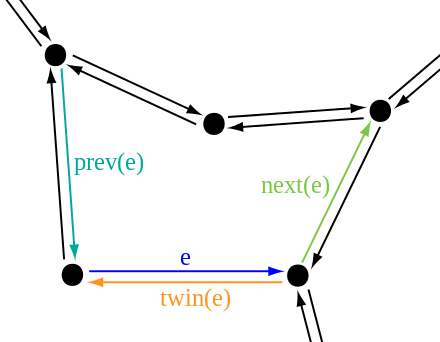
\includegraphics[scale=0.5]{images/dcel}
	\end{figure}
\end{block}

\end{frame}

\section{Horizontal Partition}
\subsection{Definition}
\begin{frame}
\begin{block}{Definition}
	The horizontal partition of an orthogonal polygon is the partition obtained after extending internally the horizontal edges of such polygon, until this extension intersects a vertical edge.
\end{block}
\end{frame}

\begin{frame}{Example}
\begin{block}{Visual Representation of a Horizontal Partition}
	\begin{figure}
		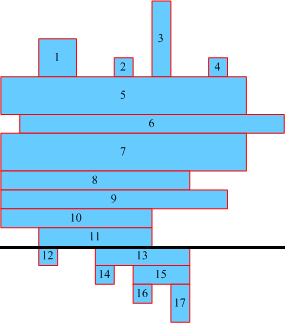
\includegraphics[scale=0.5]{images/horPartition}
	\end{figure}
\end{block}
\end{frame}

\subsection{Basic Concepts}
\begin{frame}{Basic Concepts}
\begin{block}{Geometric Primitives}
\begin{itemize}[<+->]
	\item Point;
	\item Operations between points ($+$, $-$, $\times$, $\div$);
	\item Segment;
	\item Line (equation);
	\item Polygon (set of points);
	\item CCW and CW rotations.
\end{itemize}
\end{block}
\end{frame}

\begin{frame}{Basic Concepts}
\begin{block}{Definition (Sweep Line)}
	A sweep line algorithm is an algorithmic paradigm that uses a conceptual line that is swept across the plane, stopping at some points, the \textbf{events}.
	
	\pause
	
	\bigbreak
	
	The sweep line contains, at each point, all the important information about the points, segments and others that the sweep line intersects.
	
	\pause
	
	\bigbreak
	
	At each event, we either add or remove information from the sweep line.
\end{block}

\pause

\bigbreak

In this case, each event is an horizontal edge.

\end{frame}

\subsection{Implementation}

\begin{frame}{Important Functions}
\begin{block}{\texttt{init\_poly}}
Given the points of a polygon in counterclockwise direction constructs the DCEL that represents such polygon.
\end{block}

\pause

\begin{block}{\texttt{print\_dcel}}
Prints the contents of the DCEL.
\end{block}
\end{frame}

\begin{frame}{Important Functions}
\begin{block}{\texttt{sweep\_line}}
Performs an $\mathcal{O} \left( n log \left( n \right) \right)$ horizontal sweep through the polygon.
\end{block}

\pause

\begin{block}{\texttt{init\_hole}}
Adds a hole to the DCEL representation given the points in clockwise direction.
\end{block}
\end{frame}

\begin{frame}{\texttt{splitHalfEdgeL}}

The previous functions use within themselves functions like \texttt{splitHalfEdgeL}, that given an event, if by extending it we intersect a side of the polygon and this segment lyes completely inside the polygon, divides that segment in two, creating also two different faces induced by this division. \pause It is observable that this division does not always induce two different faces (because of the holes), but since given a half-edge its next component lyes on the same face as such half-edge, \texttt{create\_face\_from} assures that they are given the same face.
	
\end{frame}

\begin{frame}{\texttt{splitHalfEdgeL}}

\begin{block}{Applications}
\begin{itemize}[<+->]
	\item If the event is from right to left, the edge of the polygon is on its left, and on the left of such event there is a piece that goes \textit{upwards} in our polygon;
	\item If the event is from left to right, the edge of the polygon is on its right, and on the right of such event there is a piece that goes \textit{downwards} in our polygon.
\end{itemize}
\end{block}

\pause

\bigbreak

\texttt{splitHalfEdgeR} can be used for the other two cases that we can get.
\end{frame}

\begin{frame}{}
	\begin{alertblock}{\texttt{map}, \texttt{set}}
	
	Since \texttt{map} and \texttt{set} are implemented as \textbf{Red-Black Trees}, this guarantees that the sweep line algorithm runs in $\mathcal{O} \left( n log \left( n \right) \right)$, since they provide the following operations:
	
	\pause
	
	\begin{itemize}[<+->]
		\item Insertion in $\mathcal{O} \left( log \left( n \right) \right)$;
		\item Deletion in $\mathcal{O} \left( log \left( n \right) \right)$;
		\item Search in $\mathcal{O} \left( log \left( n \right) \right)$.
	\end{itemize}
		
	\end{alertblock}
\end{frame}

\section{Grid Partition}
\subsection{Definition}
\begin{frame}
\begin{block}{Definition}
	The grid partition of an orthogonal polygon is the partition obtained by putting together a horizontal partition with a vertical partition.
\end{block}
\end{frame}

\begin{frame}{Example}
\begin{block}{Visual Representation of a Grid Partition}
	\begin{figure}
		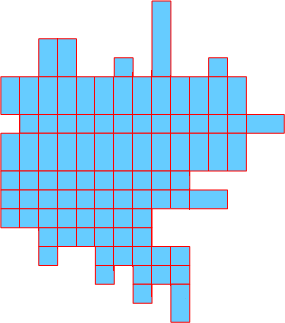
\includegraphics[scale=0.5]{images/gridPartition}
	\end{figure}
\end{block}
\end{frame}

\subsection{Idea}
\begin{frame}{Idea}
\begin{block}{First step}
The first step consists on rotating the polygon $90^{\circ}$ in CCW (we can revert this by rotating it $90^{\circ}$ in CW).

\pause

\begin{figure}
	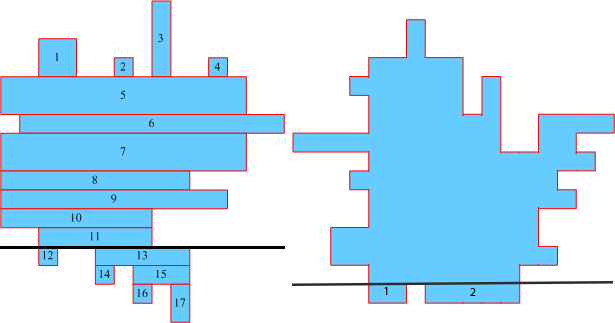
\includegraphics[scale=0.3]{images/rotatedPoly}
\end{figure}

	
\end{block}
\end{frame}

\begin{frame}{Idea}
\begin{block}{Second step}
	We semi-construct the partition induced by a horizontal sweep on such rotated polygon.
	
	\pause
	
	This semi-construction is achieved simply by storing the points of intersection of the extensions of the events with the sides of the polygon, as well as the direction of the inside half-edge, given its endpoints' vertexes' indexes (which are preserved after rotations).
\end{block}
\end{frame}

\begin{frame}{Idea}
\begin{block}{Third step}
	In the DCEL representing the horizontal partition, add these points, that we call \textbf{interest points}, to the representation, dividing the horizontal edges of the polygon accordingly.
	
	\pause
	
	\begin{figure}
		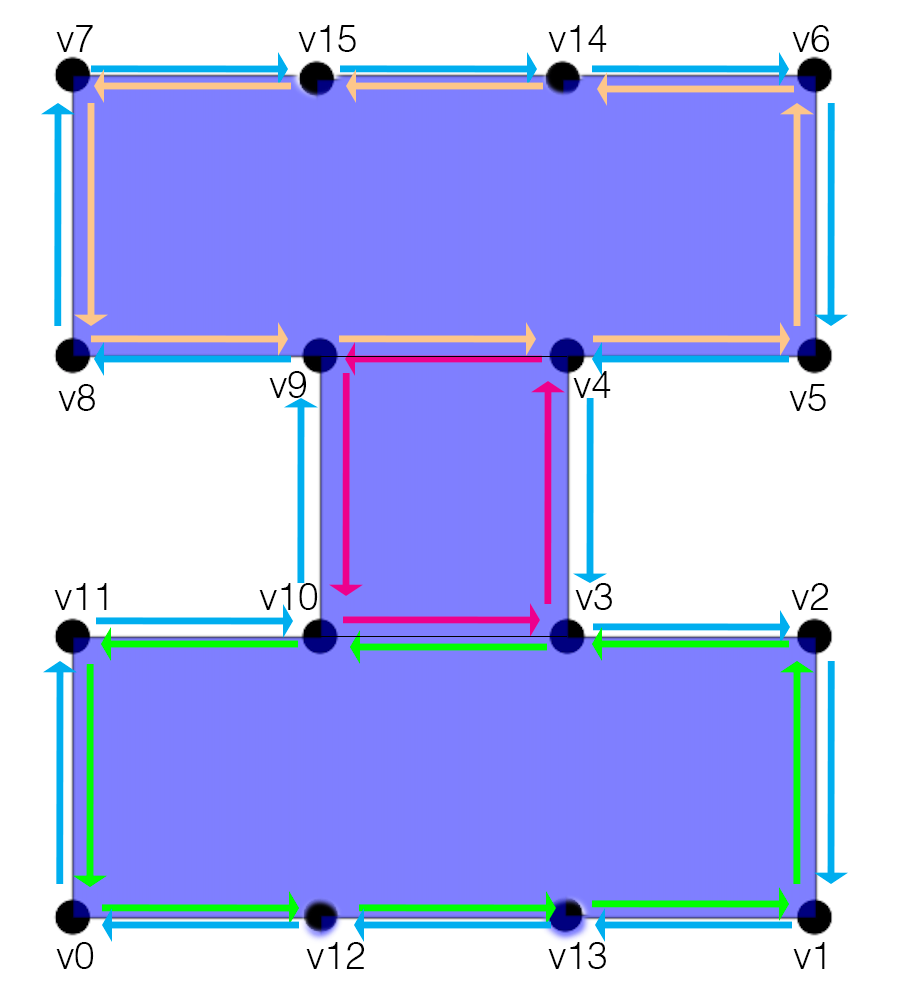
\includegraphics[scale=0.11]{images/second}
	\end{figure}
	
\end{block}
\end{frame}

\begin{frame}{Idea}
\begin{block}{Forth step}
	Since the grid partition produces faces that are rectangles, and we already have all interest points on the sides of the polygon (and on the sides of the holes, if any), we can now search for the rectangles in a way that if a face is not a rectangle, make it a rectangle. If the four endpoints of such polygon already exist, simply connect the two that are not connected, and create two new faces for each of the two faces induced by this connection. If one of the endpoints does not exist, we know that we are handling an extension of a horizontal event that needs to be divided in two.
\end{block}
\end{frame}

\section{Complexity}

\subsection{Horizontal Partition}
\begin{frame}{Horizontal Partition}

\begin{block}{Complexity}

$\mathcal{O} \left( n log \left( n \right) \right)$.
	
\end{block}

\end{frame}

\subsection{Interest Points}
\begin{frame}{Interest Points}

\begin{block}{Complexity}

$\mathcal{O} \left( n log \left( n \right) \right)$.
	
\end{block}

\end{frame}

\subsection{Grid Partition}
\begin{frame}{Grid Partition}

\begin{block}{Complexity}

Once we have the horizontal partition and the interest points, the complexity we get is $\mathcal{O} \left( n \right)$ in the number of rectangles induced by the grid partition.
	
\end{block}

\end{frame}



\end{document}
